\documentclass[11pt]{article}
\usepackage{amssymb}
\usepackage{tipa}
\usepackage{amsmath}
\usepackage[scr]{rsfso}
\usepackage{graphicx}
\usepackage{float}


\newcommand{\then}{\rightarrow} 
\newcommand{\bicond}{\leftrightarrow}
\newcommand{\powerset}[1]{\mathscr{P}(#1)}
\newcommand{\family}[1]{\mathcal{#1}}

\title{\textbf{How to Prove It} \\ {\Large\itshape Daniel J. Velleman} \\ {\Large\itshape Chapter 3.5: Proofs Involving Disjunctions}}

\author{\textbf{Nathaniel Curnick} \\ \textit{Textbook Solutions}}

\date{}

%----------------------------------------------------------------------------------------

\begin{document}

\maketitle

\section*{Exercise 1}

What are the truth sets of the following statements? List a few elements of each 
truth set.

\noindent (a) ``$x$ is a parent of $y$'', where $x$ and $y$ both range of the 
set $P$ of all people 

(Queen Elizabeth, King Charles), (King Charles, Prince William)... 

\noindent (b) ``There is someone who live in $x$ and attends $y$'', where 
$x$ ranges over the set $C$ of all cities and $y$ ranges over the set $U$ of all 
universities.

(Brighton, Sussex), (Oxford, University of Oxford)... 

\section*{Exercise 2}

What are the truth sets of the following statements? List a few elements of each 
truth set.

\noindent (a) ``$x$ lives in $y$'', where $x$ ranges over the set $P$ of all 
people and $y$ ranges over the set $C$ of all cities.

(Prince Chalres, Windsor), (Angelina Jolie, LA)... 

\noindent (b) ``The population of $x$ is $y$'', where $x$ ranges over the set $C$
of all cities and $y$ ranges over $\mathbb{N}$.

(London, 8,000,000), (Paris, 2,000,000)... 

\section*{Exercise 3}

The truth sets of the following statements are subsets of $\mathbb{R}^2$. List a 
few elements of each truth set. Draw a picture showing all the points in the plane 
whose coordinates are in the truth set 

\noindent (a) $y = x^2 - x - 2$

(0,-2), (1,-2), (2,0)... 

\begin{figure}[H]
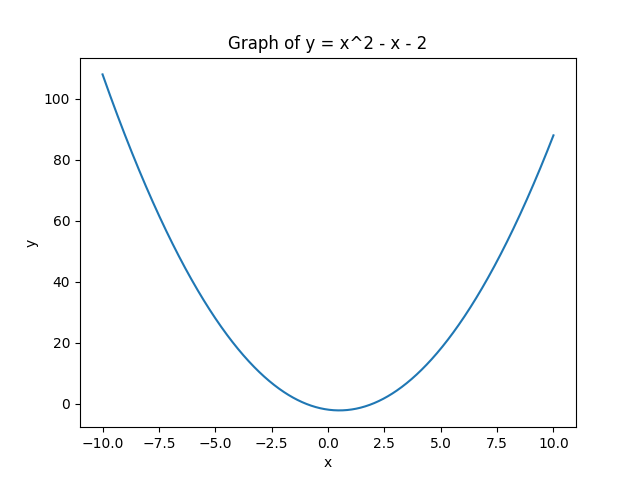
\includegraphics[width=\textwidth]{a.png}
\end{figure}

\noindent (b) $y < x$

(0, -2), (12, 3)... 

\begin{figure}[H]
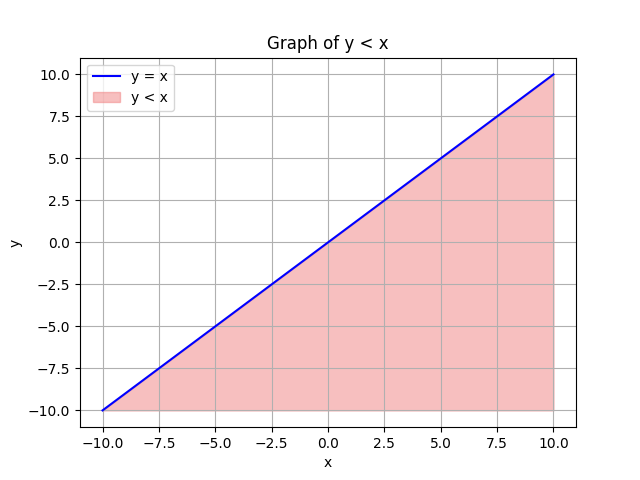
\includegraphics[width=\textwidth]{b.png}
\end{figure}

\noindent (c) Either $y = x^2 - x - 2$ or $y = 3x - 2$

\begin{figure}[H]
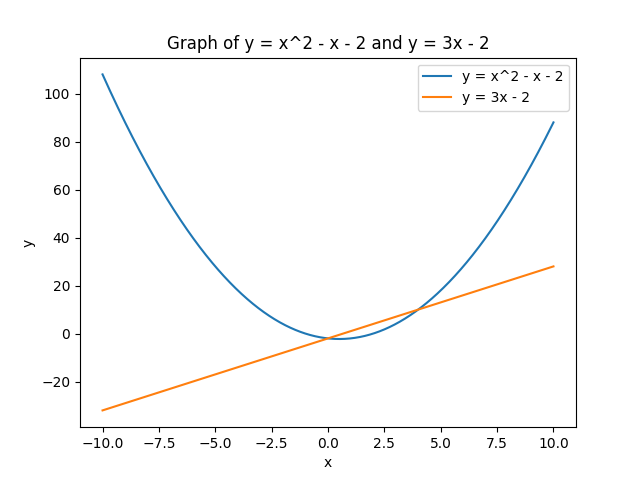
\includegraphics[width=\textwidth]{c.png}
\end{figure}

\noindent (d) $y < x$, and either $y = x^2 - x - 2$ or $y = 3x - 2$

\begin{figure}[H]
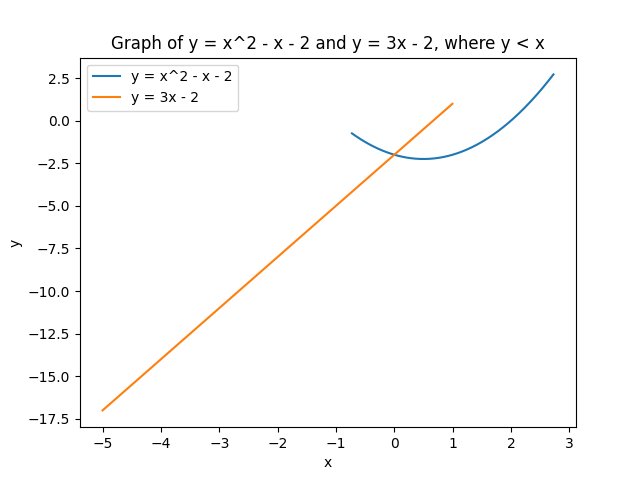
\includegraphics[width=\textwidth]{d.png}
\end{figure}

\section*{Exercise 4}

Let $A = \{ 1,2,3 \}, B = \{ 1, 4 \}, C = \{ 3,4 \}, D = \{ 5 \}$. Compute all 
the sets mentioned in Theorem 4.1.3 and verify that all parts of the theorem 
are true.

We want to demonstrate that $(A \times B) \cap (C \times D) = (A \cap C) \times (B \cap D)$

$$A \times B = \{ (1,1), (1,4), (2,1), (2,4), (3,1), (3,4) \}$$
$$C \times D = \{ (3,5), (4,5) \}$$

So 

$$(A \times B) \cap (C \times D) = \emptyset$$

Now,

$$A \cap C = \{3\}$$
$$B \cap D = \emptyset$$

So, 

$$(A \cap C) \times (B \cap D) = \emptyset$$

So we can see they are verified

\section*{Exercise 5}

Prove parts 2 and 3 of Theorem 4.1.3 

First prove $A \times (B \cup C) = (A \times B) \cup (A \times C)$

Let $p = (x,y)$ be an arbitrary element of $A \times (B \cup C)$. So, $x \in A$ 
and $y \in B \cup C$. Since $y \in B \cup C$ then $y \in B$ or $y \in C$. 
So, $(x,y) \in A \times B$ or $(x,y) \in A \times C$. Thus, 
$(x,y)=(A \times B) \cup (A \times C)$.

Now, let $p$ be an arbitrary element of $(A \times B) \cup (A \times C)$. So, 
$(x, y) \in A \times B$ or $(x, y) \in A \times C$. So, we know that $x \in A$,
the difference is in $y$. $y$ must come from either $B$ or $C$. So, 
$y \in B \cup C$. So, $(x,y) = A \times (B \cup C)$.

Now prove $(A \times B) \cap (C \times D) = (A \cap C) \times (B \cap D)$

Suppose $p = (x,y)$ and $(x,y) \in (A \times B) \cap (C \times D)$. 
So, $(x, y) \in (A \times B)$ and also at the same time $(x,y) \in (C \times D)$.
Thus, $x \in A$ and also $x \in C$. Equally, $y \in B$ and $y \in D$. Thus, 
$(x,y) \in (A \cap C) \times (B \cap D)$.

Suppose now $(x,y) \in (A \cap C) \times (B \cap D)$. So, $x \in A \cap C$ and 
$y \in B \cap D$. Since $x \in A$ and $y \in B$ then $(x,y) \in A \times B$. 
By symmetry, $(x,y) \in C \times D$. So $(x,y) = (A \times B) \cap (C \times D)$.

\section*{Exercise 6}

What's wrong with the following proof that for any sets $A, B, C, D$ that 
$(A \cup C) \times (B \cup D) \subseteq (A \times B) \cup (C \times D)$.

\textit{Proof.} Suppose $(x,y) \in (A \cup C) \times (B \cup D)$. Then 
$x \in A \cup C$ and $y \in B \cup D$, so either $x \in A$ or $x \in C$, and 
either $y \in B$ or $y \in D$. We consider these cases seperately.

Case 1. $x \in A$ and $y \in B$. Then $(x, y) \in A \times B$.

Case 2. $x \in C$ and $y \in D$. Then $(x, y) \in C \times D$.

Thus, either $(x, y) \in A \times B$ or $(x, y) \in C \times D$ so 
$(x, y) \in (A \times B) \cup (C \times D)$

\vspace{5pt}
\hrule 
\vspace{5pt}

The problem with this proof is that it leaves out some cases, namely $x \in A, 
y \in D$ and also $x \in C, y \in B$.

\section*{Exercise 7}

If $A$ has $m$ elements and $B$ has $n$ elements, how many elements does 
$A \times B$ have?

$m \times n$

\section*{Exercise 8}

Is it true that for any sets $A$, $B$ and $C$, 
$A \times (B \setminus C) = (A \times B) \setminus (A \times C)$?

It's true. Suppose $(x, y) \in A \times (B \setminus C)$. Then $x \in A$ and 
$y \in B \setminus C$, so $y \in B$ and $y \notin C$. Since $x \in A$ and $y \in B$
then $(x, y) \in A \times B$. Since $y \notin C$, $(x, y) \notin A \times C$.
Therefore $(x, y) \in (A \times B) \setminus (A \times C)$

Now suppose $(x, y) \in (A \times B) \setminus (A \times C)$. Then 
$(x, y) \in A \times B$, $x \in A$ and $y \in B$ and also 
$(x, y) \notin A \times C$, so either $x \notin A$ or $y \notin C$. But we already 
know that $x \in A$ so $y \notin C$. Since $y \in B$ and $y \notin C$, 
$y \in B \setminus C$ so $(x, y) \in A \times (B \setminus C)$

\section*{Exercise 9}

Prove that for any sets $A$, $B$, and $C$, 
$A \times (B \triangle C) = (A \times B) \setminus (A \times C)$.

$$(A \times B) \triangle (A \times C)$$
$$(A \times B) \cup (A \times C) \setminus (A \times B) \cap (A \times C)$$
$$A \times (B \cup C) \setminus A \times (B \cap C)$$
$$A \times ((B \cup C) \setminus (B \cap C))$$
$$A \times (B \triangle C)$$

\section*{Exercise 10}

Prove that for any sets $A$, $B$, $C$ and $D$, 
$(A \times B) \setminus (C \times D) \subseteq (A \times (B \setminus D) \cup (A \setminus C) \times B)$

Suppose $p = (x, y)$ and $p = (A \setminus C) \times (B \setminus D)$. 
$x \in A \setminus C$ and $y \in B \setminus D$. So, $x \in A$ and $x \notin C$
and $y \in B$ and $y \notin D$. Thus $(x, y) = A \times B$ and 
$(x, y) \notin C \times D$. So $(x, y) = (A \times B) \setminus (C \times D)$

\section*{Exercise 11}

Prove that for any sets $A$, $B$, $C$ and $D$, 
$(A \times B) \setminus (C \times D) = (A \times (B \setminus D) \cup (A \setminus C) \times B)$

Suppose $(x, y) \in (A \times B) \setminus (C \times D)$. Then $(x, y) \in A \times B$,
so $x \in A$ and $y \in B$ and also $(x, y) \notin C \times D$ so either 
$x \notin C$ or $y \notin D$.

Case 1. $x \notin C$. Then since $x \in A$ and $x \notin C$, then $x \in A \setminus C$
Since3 we also have $y \in B$ then $(x, y) \in (A \setminus C) \times B$, so 
$(x, y) \in (A \times (B \setminus D)) \cup ((A \setminus C) \times B)$

Case 2. $y \notin D$. Then since $y \in B$ and $y \notin D$, $y \in B \setminus D$.
Since we also have $x \in A$ then $(x, y) \in A \times (B \setminus D)$ so 
$(x, y) \in (A \times (B \setminus D)) \cup ((A \setminus C) \times B)$

These two cases are complete so we can conclude that 
$(x, y) \in (A \times (B \setminus D)) \cup ((A \setminus C) \times B)$ always

Now suppose $(x, y) \in (A \times (B \setminus D)) \cup ((A \setminus C) \times B)$.
Then either $(x, y) \in A \times (B \setminus D)$ or 
$(x, y) \in (A \setminus C) \times B$.

Case 1. $(x, y) \in A \times (B \setminus D)$. Then $x \in A$ and $y \in B \setminus D$
so $y \in B$ and $y \notin D$. Since $x \in A$ and $y \in B$ then 
$(x, y) \in A \times B$ and since $y \notin D$ then $(x, y) \notin C \times D$.
So, $(x, y) \in (A \times B) \setminus (C \times D)$

Case 2. $(x, y) \in (A \setminus C) \times B$. Then $x \in A \setminus C$ so 
$x \in A$ and $x \notin C$ and also $y \in B$. Since $x \in A$ and $y \in B$
then $(x, y) \in A \times B$ and since $x \notin C$ then $(x, y) \notin C \times D$.
Therefore $(x, y) \in (A \times B) \setminus (C \times D)$

Thus, $(x, y) \in (A \times B) \setminus (C \times D)$

\section*{Exercise 12}

Prove that for any sets $A$, $B$, $C$ and $D$, if $A \times B$ and $C \times D$ 
are disjoint then either $A$ and $C$ are disjoint or $B$ and $D$ are disjoint

Converting this into mathematical notation we need to show that if 
$(A \times D) \cap (C \times D) = \emptyset \then (A \cap C = \emptyset) \cup 
(B \cap D = \emptyset)$

Suppose $(x, y) = A \times B$. Since $A \times B \cap C \times D = \emptyset$
then $(x, y) \notin C \times D$. Since $x \in A$ and $y \in B$ then we can say 
$x \notin C$ and $y \notin D$. Thus $A \cap C = \emptyset$ or $B \cap D = \emptyset$

If instead $(x, y) = C \times D$ the same argument applies by symmetry: 
$x \in C$, $x \notin A$, $A \cap C = \emptyset$. $y \in D$, $y \notin B$,
$B \cap D = \emptyset$.

\section*{Exercise 13}

Suppose $I \neq \emptyset$. Prove that for any indexed family of sets 
$\{ A_i | i \in I\}$ and any sets $B$, 
$(\bigcap_{i \in I} A_i) \times B = \bigcap_{i \in I} (A_i \times B)$.
Where in the proof does the assumption $I \neq \emptyset$ used?

Let $(x, y) = (\bigcap_{i \in I} A_i) \times B$. We can see that $y \in B$. 
Also $x \in \bigcap_{i \in I} A_i$. We can choose some arbitrary $i_0 \in I$ 
(this is where we use $I \neq \emptyset$) and say 
$(x, y) = A_{i_0} \times B$. But since $i_0$ was arbitrary then 
$(x, y) = \bigcap_{i \in I} (A_i \times B)$. Now suppose 
$(x, y) = \bigcap_{i \in I} (A_i \times B)$. If we choose some arbitrary $i_0 \in I$
then we can see $(x, y) = A_{i_0} \times B$. So $x \in A_{i_0}$ and $y \in B$. But 
since $i_0$ was arbitrary then we can say $(x, y) = (\bigcap_{i \in I} A_i) \times B$

\section*{Exercise 14}

Suppose $\{A_i | i \in I\}$ and $\{B_i | i \in I\}$ are indexed families of sets 

\noindent (a) Prove that $\bigcup_{i \in I} (A_i \times B_i) \subseteq 
(\bigcup_{i \in I} A_i) \times (\bigcup_{i \in I} B_i)$

Suppose $(x, y) = \bigcup_{i \in I} (A_i \times B_i)$. Choose some $i_0 \in I$.
Then $(x, y) = A_{i_0} \times B_{i_0}$. We can see that $x \in A_{i_0}$ and 
$y \in B_{i_0}$. But since $i_0$ was arbitrary we can also say that 
$x \in \bigcup_{i \in I} A_i$ and $y \in \bigcup_{i \in I} B_i$. Or in other words 
$(x, y) = \bigcup_{i \in I} A_i \times \bigcup_{i \in I} B_i$

\noindent (b) For each $(i, j) \in I \times I$ let $C_{(i, j)} = A_i \times B_j$
and let $P = I \times I$. Prove that $\bigcup_{p \in P} C_p = (\bigcup_{i \in I} A_i) \times (\bigcup_{i \in I} B_i)$

Suppose $(x, y) \in \bigcup_{p \in P} C_p$. Then we choose $(i_0, i_1) \in P = I \times I$
such that $(x, y) \in C_{i_0, i_1} = A_{i_0} \times B_{i_1}$. Therefore $x \in A_{i_0}$
and $y \in B_{i_1}$ so $x \in \bigcup_{i \in I} A_i$ and $y \in \bigcup_{i \in I} B_i$
and thus $(x, y) \in (\bigcup_{i \in I} A_i) \times (\bigcup_{i \in I} B_i)$.
Now suppose $(x, y) \in \bigcup_{i \in I} A_i \times \bigcup_{i \in I} B_i$ then 
$x \in \bigcup_{i \in I} A_i$ and $y \in \bigcup_{i \in I} B_i$ so we can choose 
$i_0$ and $i_1$ in $I$ such that $x \in A_{i_0}$ and $y \in B_{i_1}$. Therefore 
$(x, y) \in A_{i_0} \times B_{i_1}$. Therefore $(x, y) \in A_{i_0} \times B_{i_1}$.
Therefore $(x, y) \in A_{i_0} \times B_{i_1} = C_{i_0, i_1}$ and $i_0, i_1 = I \times I = P$
so $(x, y) \in \bigcup_{p \in P} C_p$

\section*{Exercise 15}

This problem was suggested by Professor Alan Taylor of Union College, NY. consider 
the following putative theorem.

\textbf{Theorem?} For any sets $A$, $B$, $C$ and $D$ if $A \times B \subseteq C \times D$ 
then $A \subseteq C$ and $B \subseteq D$.

Is the following proof correct? If so, what proof strategies does it use? If not,
can it be fixed? Is the theorem correct?

\textit{Proof?} Suppose $A \times B \subseteq C \times D$. Let $a$ be an arbitrary
element of $A$ and let $b$ be an arbitrary element of $B$. Then $(a, b) \in A \times B$, 
so since $A \times B \subseteq C \times D$, $(a, b) \in C \times D$. Therefore 
$a \in C$ and $b \in D$. Since $a$ and $b$ were arbitrary elements of $A$ and 
$B$ respectively this shows that $A \subseteq C$ and $B \subseteq D$.

The theorem itself is incorrect.

A counterexample is $A = \{1\}, B = C = D = \emptyset$.

The problem with this proof is that it tries to prove $A \subseteq C$ and 
$B \subseteq D$ in one fell swoop when they need seperate proofs.





\end{document}
